\documentclass[10pt,a4paper]{article}
\usepackage[UTF8,fontset = windows]{ctex}
\setCJKmainfont[BoldFont=黑体,ItalicFont=楷体]{华文中宋}
\usepackage{amssymb,amsmath,amsfonts,amsthm,mathrsfs,dsfont,graphicx}
\usepackage{ifthen,indentfirst,enumerate,color,titletoc}
\usepackage{tikz}
\usepackage{multicol}
\usepackage{makecell}
\usepackage{longtable}
\usetikzlibrary{arrows,calc,intersections,patterns,decorations.pathreplacing,3d,angles,quotes,positioning}
\usepackage[bf,small,indentafter,pagestyles]{titlesec}
\usepackage[top=1in, bottom=1in,left=0.8in,right=0.8in]{geometry}
\renewcommand{\baselinestretch}{1.65}
\newtheorem{defi}{定义~}
\newtheorem{eg}{例~}
\newtheorem{ex}{~}
\newtheorem{rem}{注~}
\newtheorem{thm}{定理~}
\newtheorem{coro}{推论~}
\newtheorem{axiom}{公理~}
\newtheorem{prop}{性质~}
\newcommand{\blank}[1]{\underline{\hbox to #1pt{}}}
\newcommand{\bracket}[1]{(\hbox to #1pt{})}
\newcommand{\onech}[4]{\par\begin{tabular}{p{.9\textwidth}}
A.~#1\\
B.~#2\\
C.~#3\\
D.~#4
\end{tabular}}
\newcommand{\twoch}[4]{\par\begin{tabular}{p{.46\textwidth}p{.46\textwidth}}
A.~#1& B.~#2\\
C.~#3& D.~#4
\end{tabular}}
\newcommand{\vartwoch}[4]{\par\begin{tabular}{p{.46\textwidth}p{.46\textwidth}}
(1)~#1& (2)~#2\\
(3)~#3& (4)~#4
\end{tabular}}
\newcommand{\fourch}[4]{\par\begin{tabular}{p{.23\textwidth}p{.23\textwidth}p{.23\textwidth}p{.23\textwidth}}
A.~#1 &B.~#2& C.~#3& D.~#4
\end{tabular}}
\newcommand{\varfourch}[4]{\par\begin{tabular}{p{.23\textwidth}p{.23\textwidth}p{.23\textwidth}p{.23\textwidth}}
(1)~#1 &(2)~#2& (3)~#3& (4)~#4
\end{tabular}}
\begin{document}

\begin{enumerate}[1.]


\item{ (004164)}集合$A=\{x|x^2-2x<0\}$, $B=\{x||x|<1\}$, 则$A\cup B$=\blank{50}.


关联目标:

K0104004B|D01001B|能用文氏图反映两个集合的并集.



标签: 第一单元

答案: $(-1,2)$

解答或提示: 暂无解答与提示

使用记录:

20220421	2022届高三1班	\fcolorbox[rgb]{0,0,0}{1.000,0.140,0}{0.930}

20220821	2023届高三2班	\fcolorbox[rgb]{0,0,0}{1.000,0.122,0}{0.939}

20220821	2023届高三3班	\fcolorbox[rgb]{0,0,0}{1.000,0.334,0}{0.833}

20220821	2023届高三10班	\fcolorbox[rgb]{0,0,0}{1.000,0.250,0}{0.875}

20220821	2023届高三9班	\fcolorbox[rgb]{0,0,0}{1.000,0.388,0}{0.806}

20220821	2023届高三12班	\fcolorbox[rgb]{0,0,0}{1.000,0.500,0}{0.750}


出处: 2022届高三下学期测验卷06第1题
\newpage
\item{ (007684)}用适当的方法表示下列集合:\\
(1) 方程$x^2-2=0$的实数解组成的集合;\\
(2) 两直线$y=2x+1$和$y=x-2$的交点组成的集合.


关联目标:

K0102003B|D01001B|会选择合适的表示集合的方式, 会正确地进行表示方式的切换.



标签: 第一单元

答案: (1) $\{-\sqrt{2},\sqrt{2}\}$; (2) $\{(-3,-5)\}$

解答或提示: 暂无解答与提示

使用记录:

20220821	2023届高三2班	\fcolorbox[rgb]{0,0,0}{1.000,0.000,0}{1.000}	\fcolorbox[rgb]{0,0,0}{1.000,0.000,0}{1.000}

20220821	2023届高三3班	\fcolorbox[rgb]{0,0,0}{1.000,0.334,0}{0.833}	\fcolorbox[rgb]{0,0,0}{1.000,0.166,0}{0.917}

20220821	2023届高三10班	\fcolorbox[rgb]{0,0,0}{1.000,0.166,0}{0.917}	\fcolorbox[rgb]{0,0,0}{1.000,0.250,0}{0.875}

20220821	2023届高三9班	\fcolorbox[rgb]{0,0,0}{1.000,0.322,0}{0.839}

20220821	2023届高三12班	\fcolorbox[rgb]{0,0,0}{1.000,0.166,0}{0.917}


出处: 二期课改练习册高一第一学期
\newpage
\item{ (004781)}已知集合$A=\{x|\dfrac{12}{5-x}\in \mathbf{N},\ x\in\mathbf{Z}\}$, 用列举法表示集合$A$.


关联目标:

K0101001B|D01001B|通过具体的例子理解集合的含义, 理解元素与集合的``属于''关系, 并能用符号表示.

K0102001B|D01001B|能在具体情境中用列举法表示集合.



标签: 第一单元

答案: $\{-7,-1,1,2,3,4\}$

解答或提示: 暂无解答与提示

使用记录:

20220821	2023届高三2班	\fcolorbox[rgb]{0,0,0}{1.000,0.242,0}{0.879}

20220821	2023届高三3班	\fcolorbox[rgb]{0,0,0}{1.000,0.500,0}{0.750}

20220821	2023届高三10班	\fcolorbox[rgb]{0,0,0}{1.000,0.334,0}{0.833}

20220821	2023届高三9班	\fcolorbox[rgb]{0,0,0}{1.000,0.322,0}{0.839}

20220821	2023届高三12班	\fcolorbox[rgb]{0,0,0}{1.000,0.334,0}{0.833}


出处: 代数精编第一章集合与命题
\newpage
\item{ (007692)}已知$a$是常数, 集合$M=\{x|x^2+x-6=0\}$, 集合$N=\{y|ay+2=0\}$, 且$N\subseteq M$, 求实数$a$的值.


关联目标:

K0101002B|D01001B|理解有限集、无限集、空集的含义.



标签: 第一单元

答案: $0$或$-1$或$\dfrac 23$

解答或提示: 暂无解答与提示

使用记录:

20220821	2023届高三2班	\fcolorbox[rgb]{0,0,0}{1.000,0.242,0}{0.879}

20220821	2023届高三3班	\fcolorbox[rgb]{0,0,0}{1.000,0.416,0}{0.792}

20220821	2023届高三10班	\fcolorbox[rgb]{0,0,0}{1.000,0.416,0}{0.792}

20220821	2023届高三9班	\fcolorbox[rgb]{0,0,0}{1.000,0.646,0}{0.677}

20220821	2023届高三12班	\fcolorbox[rgb]{0,0,0}{1.000,0.916,0}{0.542}


出处: 二期课改练习册高一第一学期
\newpage
\item{ (002693)}已知$P=\{y=x^2+1\}$, $Q=\{y|y=x^2+1, \ x\in \mathbf{R}\}$, $E=\{x|y=x^2+1, \  x\in \mathbf{R}\}$, $F=\{(x,y)|y=x^2+1, \ x\in \mathbf{R}\}$, $G=\{x|x\ge 1\}$, $H=\{x|x^2+1=0, \ x\in \mathbf{R}\}$, 则各集合间关系正确的有\blank{50}. (答案可能不唯一)\\
\textcircled{1} $P=F$; \textcircled{2} $Q=E$; \textcircled{3} $E=F$; \textcircled{4} $Q\subseteq G$; \textcircled{5} $H\subset P$.


关联目标:

K0101004B|D01001B|知道集合相等的定义.

K0103001B|D01001B|理解集合之间包含的概念, 能识别给定集合的子集.



标签: 第一单元

答案: \textcircled{4}\textcircled{5}

解答或提示: 暂无解答与提示

使用记录:

20220821	2023届高三2班	\fcolorbox[rgb]{0,0,0}{1.000,0.910,0}{0.545}

20220821	2023届高三3班	\fcolorbox[rgb]{0,0,0}{1.000,0.916,0}{0.542}

20220821	2023届高三10班	\fcolorbox[rgb]{0,0,0}{1.000,0.334,0}{0.833}

20220821	2023届高三9班	\fcolorbox[rgb]{0,0,0}{0.968,1.000,0}{0.484}

20220821	2023届高三12班	\fcolorbox[rgb]{0,0,0}{0.916,1.000,0}{0.458}


出处: 2022届高三第一轮复习讲义
\newpage
\item{ (002728)}设含有三个实数的集合既可以表示为$\{a,\dfrac ba,1\}$, 又可以表示为$\{a^2,a+b,0\}$, 那么$a+b=$\blank{50}.


关联目标:

K0101004B|D01001B|知道集合相等的定义.



标签: 第一单元

答案: $-1$

解答或提示: 暂无解答与提示

使用记录:

20220821	2023届高三2班	\fcolorbox[rgb]{0,0,0}{1.000,0.122,0}{0.939}

20220821	2023届高三3班	\fcolorbox[rgb]{0,0,0}{1.000,0.334,0}{0.833}

20220821	2023届高三10班	\fcolorbox[rgb]{0,0,0}{1.000,0.250,0}{0.875}

20220821	2023届高三9班	\fcolorbox[rgb]{0,0,0}{1.000,0.710,0}{0.645}

20220821	2023届高三12班	\fcolorbox[rgb]{0,0,0}{1.000,0.416,0}{0.792}


出处: 2022届高三第一轮复习讲义
\newpage
\item{ (002704)}(1) 已知集合$A=\{y|y=x^2, \ x\in \mathbf{R}\}, B=\{y|y=4-x^2, \ x\in \mathbf{R}\}$, 则$A\cap B=$\blank{50}.\\
(2) 已知集合$A=\{(x,y)|y={x^2},\ x\in \mathbf{R}\}$, $B=\{(x,y)|y=4-x^2, \ x\in \mathbf{R}\}$, 则$A\cap B=$\blank{50}.


关联目标:

K0102002B|D01001B|能在具体情境中用描述法表示集合.

K0102003B|D01001B|会选择合适的表示集合的方式, 会正确地进行表示方式的切换.



标签: 第一单元

答案: (1) $[0,4]$; (2) $\{(-\sqrt{2},2),(\sqrt{2},2)\}$

解答或提示: 暂无解答与提示

使用记录:

20220821	2023届高三2班	\fcolorbox[rgb]{0,0,0}{1.000,0.364,0}{0.818}	\fcolorbox[rgb]{0,0,0}{1.000,0.242,0}{0.879}

20220821	2023届高三3班	\fcolorbox[rgb]{0,0,0}{1.000,0.416,0}{0.792}	\fcolorbox[rgb]{0,0,0}{1.000,0.166,0}{0.917}

20220821	2023届高三10班	\fcolorbox[rgb]{0,0,0}{1.000,0.916,0}{0.542}	\fcolorbox[rgb]{0,0,0}{1.000,0.334,0}{0.833}

20220821	2023届高三9班	\fcolorbox[rgb]{0,0,0}{1.000,0.646,0}{0.677}	\fcolorbox[rgb]{0,0,0}{1.000,0.322,0}{0.839}

20220821	2023届高三12班	\fcolorbox[rgb]{0,0,0}{1.000,0.834,0}{0.583}


出处: 2022届高三第一轮复习讲义
\newpage
\item{ (020030)}设常数$a\in \mathbf{R}$. 若集合$A=(-\infty ,5)$与$B=(-\infty ,a]$满足$A\subseteq B$, 则$a$的取值范围是\blank{50}.\\
证明: $1^\circ$ 当$a$\blank{50}时, 任取$x\in A$, 则\blank{50}, 所以$x\in B$, 即$A\subseteq B$.\\ 
$2^\circ$ 当$a$\blank{50}时, 取$x_1=$\blank{50}, 则\blank{50}, 所以$x_1\in A$且$x_1\not \in B$.\\
由$1^\circ$、$2^\circ$可得结论.


关联目标:

K0103001B|D01001B|理解集合之间包含的概念, 能识别给定集合的子集.



标签: 第一单元

答案: $[5,+\infty)$; $\ge 5$; $x<5<a$; $x<5$, $\dfrac{5+a}2$; $a<x_1<5$.

解答或提示: 暂无解答与提示

使用记录:

20220821	2023届高三2班	\fcolorbox[rgb]{0,0,0}{0.364,1.000,0}{0.182}

20220821	2023届高三3班	\fcolorbox[rgb]{0,0,0}{1.000,1.000,0}{0.500}

20220821	2023届高三10班	\fcolorbox[rgb]{0,0,0}{1.000,0.570,0}{0.715}

20220821	2023届高三9班	\fcolorbox[rgb]{0,0,0}{0.000,1.000,0}{0.000}

20220821	2023届高三12班	\fcolorbox[rgb]{0,0,0}{0.000,1.000,0}{0.000}


出处: 2025届高一校本作业必修第一章
\newpage
\item{ (002716)}已知集合$M=\{x|x=3m+1, \ m\in \mathbf{Z}\}$, $N=\{y|y=3m+2, \ m\in \mathbf{Z}\}$, 若$x_0\in M$, $y_0\in N$, 则$x_0y_0$与集合$M,N$的关系是\bracket{20}.
\twoch{$x_0y_0\in M$但$x_0y_0$$\notin N$}{$x_0y_0\in N$但$x_0y_0\notin M$}{$x_0y_0\notin M$且$x_0y_0\notin N$}{$x_0y_0$$\in M$且$x_0y_0\in N$}


关联目标:

K0101001B|D01001B|通过具体的例子理解集合的含义, 理解元素与集合的``属于''关系, 并能用符号表示.



标签: 第一单元

答案: B

解答或提示: 暂无解答与提示

使用记录:

20220821	2023届高三2班	\fcolorbox[rgb]{0,0,0}{1.000,0.182,0}{0.909}

20220821	2023届高三3班	\fcolorbox[rgb]{0,0,0}{1.000,0.334,0}{0.833}

20220821	2023届高三10班	\fcolorbox[rgb]{0,0,0}{1.000,0.584,0}{0.708}

20220821	2023届高三9班	\fcolorbox[rgb]{0,0,0}{1.000,0.388,0}{0.806}

20220821	2023届高三12班	\fcolorbox[rgb]{0,0,0}{1.000,0.500,0}{0.750}


出处: 2022届高三第一轮复习讲义
\newpage
\item{ (002710)}如图, $U$为全集, $M,P,S$是$U$的三个子集, 则阴影部分所表示的集合是\bracket{20}.
\begin{center}
    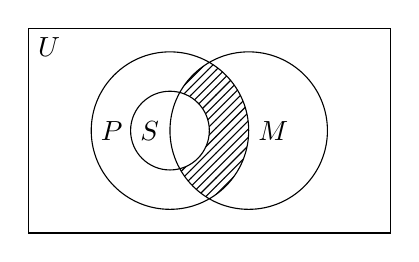
\begin{tikzpicture}
        \begin{scope}
            \clip (1,0) circle (1);
            \begin{scope}[even odd rule]
                \clip (0,0) circle (1) (0,0) circle (0.5);
                \filldraw [pattern = {north east lines}] (-2,-2) rectangle (2,2);
            \end{scope}
        \end{scope}
        \draw (0,0) circle (1) (1,0) circle (1) (0,0) circle (0.5);
        \draw (-1.8,-1.3) rectangle (2.8,1.3);
        \draw (-1.8,1.3) node [below right] {$U$} (-1,0) node [right] {$P$} (-0.5,0) node [right] {$S$} (1,0) node [right] {$M$};
    \end{tikzpicture}
\end{center}
\fourch{$(M\cap P)\cap S$}{$(M\cap P)\cup S$}{$(M\cap P)\cap \overline S$}{$(M\cap P)\cup \overline S$}


关联目标:

K0104002B|D01001B|能用文氏图反映两个集合的交集.

K0104004B|D01001B|能用文氏图反映两个集合的并集.

K0104007B|D01001B|能用文氏图反映一个集合的补集.



标签: 第一单元

答案: C

解答或提示: 暂无解答与提示

使用记录:

20220821	2023届高三2班	\fcolorbox[rgb]{0,0,0}{1.000,0.122,0}{0.939}

20220821	2023届高三3班	\fcolorbox[rgb]{0,0,0}{1.000,0.084,0}{0.958}

20220821	2023届高三10班	\fcolorbox[rgb]{0,0,0}{1.000,0.084,0}{0.958}

20220821	2023届高三9班	\fcolorbox[rgb]{0,0,0}{1.000,0.064,0}{0.968}

20220821	2023届高三12班	\fcolorbox[rgb]{0,0,0}{1.000,0.000,0}{1.000}


出处: 2022届高三第一轮复习讲义
\newpage
\item{ (002702)}若集合$A=[2,3]$, 集合$B=[a,2a+1]$.\\
(1) 若$A\subset B$, 求实数$a$的取值范围;\\
(2) 若$A\cap B\ne \varnothing$, 求实数$a$的取值范围.


关联目标:

K0102004B|D01001B|会用区间表示一些实数集合.

K0103005B|D01001B|理解真子集的概念, 能在具体的例子中证明给定集合间的真子集关系.



标签: 第一单元

答案: (1) $[1,2]$; (2) $[\dfrac 12 3]$.

解答或提示: 暂无解答与提示

使用记录:

20220821	2023届高三2班	\fcolorbox[rgb]{0,0,0}{0.424,1.000,0}{0.212}	\fcolorbox[rgb]{0,0,0}{0.666,1.000,0}{0.333}

20220821	2023届高三3班	\fcolorbox[rgb]{0,0,0}{0.666,1.000,0}{0.333}	\fcolorbox[rgb]{0,0,0}{0.666,1.000,0}{0.333}

20220821	2023届高三10班	\fcolorbox[rgb]{0,0,0}{0.416,1.000,0}{0.208}	\fcolorbox[rgb]{0,0,0}{1.000,0.416,0}{0.792}

20220821	2023届高三9班	\fcolorbox[rgb]{0,0,0}{0.968,1.000,0}{0.484}	\fcolorbox[rgb]{0,0,0}{1.000,0.516,0}{0.742}

20220821	2023届高三12班	\fcolorbox[rgb]{0,0,0}{0.666,1.000,0}{0.333}


出处: 2022届高三第一轮复习讲义
\newpage
\item{ (004768)}已知集合$U =\{x|x\text{取不大于}30\text{的质数}\}$, $A$, $B$是$U$的两个子集, 且满足$A\cap \overline B=\{5,13,23\}$, $\overline A\cap B=\{11,19,29\}$, $\overline A\cap \overline B=\{3,7\}$, 求$A$, $B$.


关联目标:

K0104002B|D01001B|能用文氏图反映两个集合的交集.

K0104004B|D01001B|能用文氏图反映两个集合的并集.

K0104007B|D01001B|能用文氏图反映一个集合的补集.



标签: 第一单元

答案: $A=\{2,5,13,17,23\}$, $B=\{2,11,17,19,29\}$

解答或提示: 暂无解答与提示

使用记录:

20220821	2023届高三2班	\fcolorbox[rgb]{0,0,0}{1.000,0.122,0}{0.939}

20220821	2023届高三3班	\fcolorbox[rgb]{0,0,0}{1.000,0.166,0}{0.917}

20220821	2023届高三10班	\fcolorbox[rgb]{0,0,0}{1.000,0.000,0}{1.000}

20220821	2023届高三9班	\fcolorbox[rgb]{0,0,0}{1.000,0.194,0}{0.903}

20220821	2023届高三12班	\fcolorbox[rgb]{0,0,0}{1.000,0.250,0}{0.875}


出处: 代数精编第一章集合与命题
\newpage
\item{ (010027)}已知集合$A=\{x|x=2n+1,\ n\in \mathbf{Z}\}$, $B=\{x|x=4n-1,\ n\in \mathbf{Z}\}$. 判断集合$A$与$B$的包含关系, 并证明你的结论.


关联目标:

K0103001B|D01001B|理解集合之间包含的概念, 能识别给定集合的子集.

K0103003B|D01001B|能在简单的情境中, 证明集合间的子集关系.



标签: 第一单元

答案: $B\subset A$, 证明略

解答或提示: 暂无解答与提示

使用记录:

20220821	2023届高三2班	\fcolorbox[rgb]{0,0,0}{1.000,0.848,0}{0.576}

20220821	2023届高三3班	\fcolorbox[rgb]{0,0,0}{1.000,0.584,0}{0.708}

20220821	2023届高三10班	\fcolorbox[rgb]{0,0,0}{1.000,0.708,0}{0.646}

20220821	2023届高三9班	\fcolorbox[rgb]{0,0,0}{0.646,1.000,0}{0.323}

20220821	2023届高三12班	\fcolorbox[rgb]{0,0,0}{0.500,1.000,0}{0.250}


出处: 新教材必修第一册习题
\newpage
\item{ (020035)}证明:集合$A=\{x|x=6n-1, \ n\in\mathbf{Z}\}$是$B=\{x|x=3n+2, \ n\in\mathbf{Z}\}$的真子集.


关联目标:

K0103005B|D01001B|理解真子集的概念, 能在具体的例子中证明给定集合间的真子集关系.



标签: 第一单元

答案: 证明略

解答或提示: 暂无解答与提示

使用记录:

20220821	2023届高三2班	\fcolorbox[rgb]{0,0,0}{1.000,0.788,0}{0.606}

20220821	2023届高三3班	\fcolorbox[rgb]{0,0,0}{1.000,0.416,0}{0.792}

20220821	2023届高三10班	\fcolorbox[rgb]{0,0,0}{1.000,0.792,0}{0.604}

20220821	2023届高三9班	\fcolorbox[rgb]{0,0,0}{0.774,1.000,0}{0.387}

20220821	2023届高三12班	\fcolorbox[rgb]{0,0,0}{0.666,1.000,0}{0.333}


出处: 2025届高一校本作业必修第一章
\newpage
\item{ (001003)}已知集合$A=\{1,2\}$, $B=\{x|x^2-ax+a-1=0,\ x\in\mathbf{R}\}$, 若$B$不是$A$的真子集, 求实数$a$的值.


关联目标:

K0103005B|D01001B|理解真子集的概念, 能在具体的例子中证明给定集合间的真子集关系.



标签: 第一单元

答案: $\{x|x\ne 2, \ x\in \mathbf{R}\}$

解答或提示: 暂无解答与提示

使用记录:

2016届11班	\fcolorbox[rgb]{0,0,0}{1.000,0.974,0}{0.513}

2016届12班	\fcolorbox[rgb]{0,0,0}{1.000,0.894,0}{0.553}

20220821	2023届高三2班	\fcolorbox[rgb]{0,0,0}{0.728,1.000,0}{0.364}

20220821	2023届高三3班	\fcolorbox[rgb]{0,0,0}{1.000,0.834,0}{0.583}

20220821	2023届高三10班	\fcolorbox[rgb]{0,0,0}{0.876,1.000,0}{0.438}

20220821	2023届高三9班	\fcolorbox[rgb]{0,0,0}{0.710,1.000,0}{0.355}

20220821	2023届高三12班	\fcolorbox[rgb]{0,0,0}{0.500,1.000,0}{0.250}


出处: 2016届创新班作业	1105-集合的关系
\newpage
\item{ (001015)}已知集合$A=\{x|\ x^2+px+q=0\}$, $B=\{x|\ x^2-x+r=0\}$, 且$A\cap B=\{-1\}$, $A\cup B=\{-1,2\}$, 求实数$p,q,r$的值.


关联目标:

K0104001B|D01001B|理解两个集合的交集的含义, 在具体数学情境中, 能求两个集合的交集.

K0104003B|D01001B|理解两个集合的并集的含义, 在具体数学情境中, 能求两个集合的并集.



标签: 第一单元

答案: $p=2$, $q=1$, $r=-2$

解答或提示: 暂无解答与提示

使用记录:

2016届11班	\fcolorbox[rgb]{0,0,0}{1.000,0.666,0}{0.667}

2016届12班	\fcolorbox[rgb]{0,0,0}{1.000,0.820,0}{0.590}

20220821	2023届高三2班	\fcolorbox[rgb]{0,0,0}{1.000,0.484,0}{0.758}

20220821	2023届高三3班	\fcolorbox[rgb]{0,0,0}{1.000,0.250,0}{0.875}

20220821	2023届高三10班	\fcolorbox[rgb]{0,0,0}{1.000,0.292,0}{0.854}

20220821	2023届高三9班	\fcolorbox[rgb]{0,0,0}{1.000,0.388,0}{0.806}

20220821	2023届高三12班	\fcolorbox[rgb]{0,0,0}{1.000,0.500,0}{0.750}


出处: 2016届创新班作业	1106-集合的运算
\end{enumerate}



\end{document}